\chapter{Results}
\label{chap:results}

%introdution to results and the likelihood definition here

\begin{figure}[hptb]
\centering
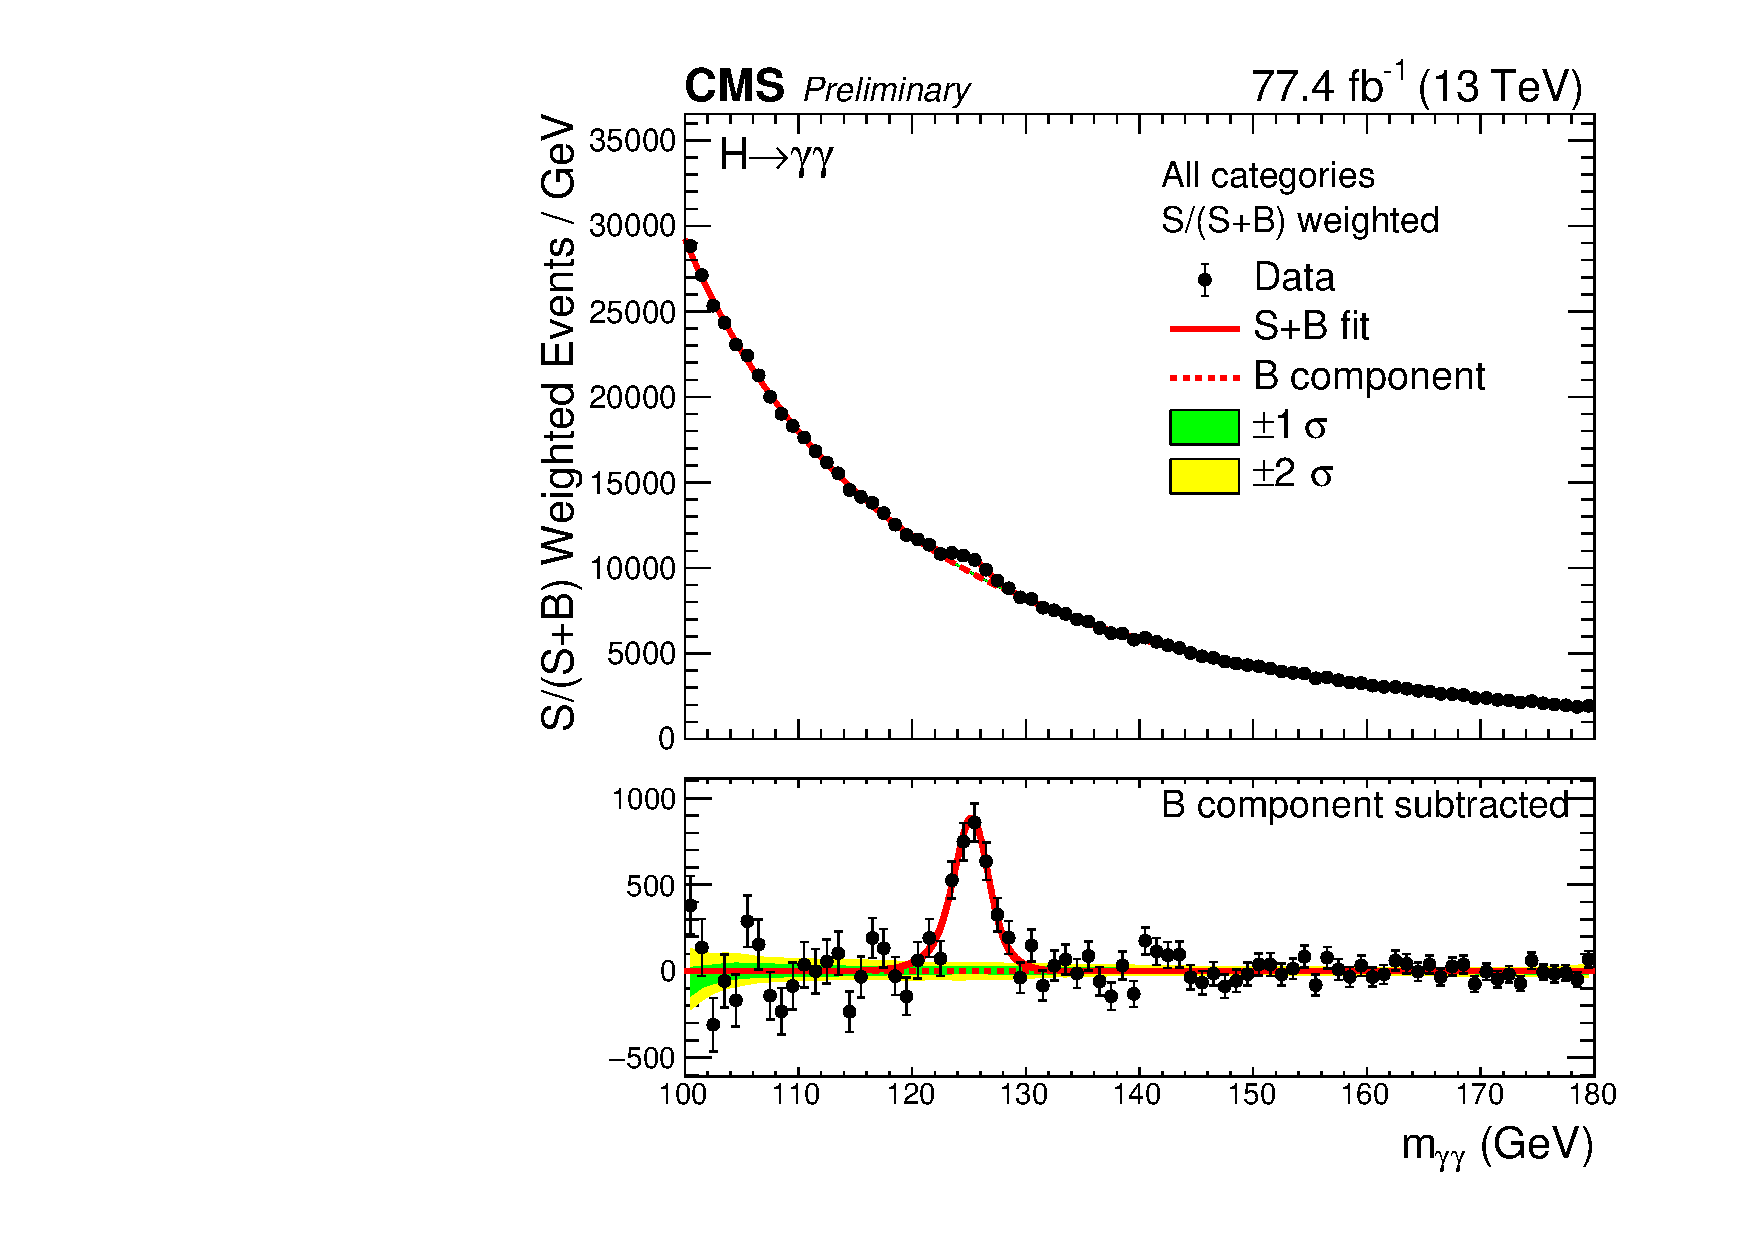
\includegraphics[width=\textwidth]{Figures/Results/MassPlot.pdf}
\caption{
  Data points (black) and signal plus background model fit for the sum of all categories is shown. 
  Each category is weighted by S/(S + B), 
  where S and B are the numbers of expected signal and background events, respectively, 
  in a $\pm 1 \seff$ mass window centered on \mH. 
  The one standard deviation (green) and two standard deviation (yellow) bands 
  include the uncertainties in the background component of the fit. 
  The solid red line shows the contribution from the total signal, plus the background contribution. 
  The dashed red line shows the contribution from the background component of the fit. 
  The bottom plot shows the residuals after subtraction of this background component.
}
\label{fig:results_MassPlot}
\end{figure}

\begin{figure}[hptb]
\centering
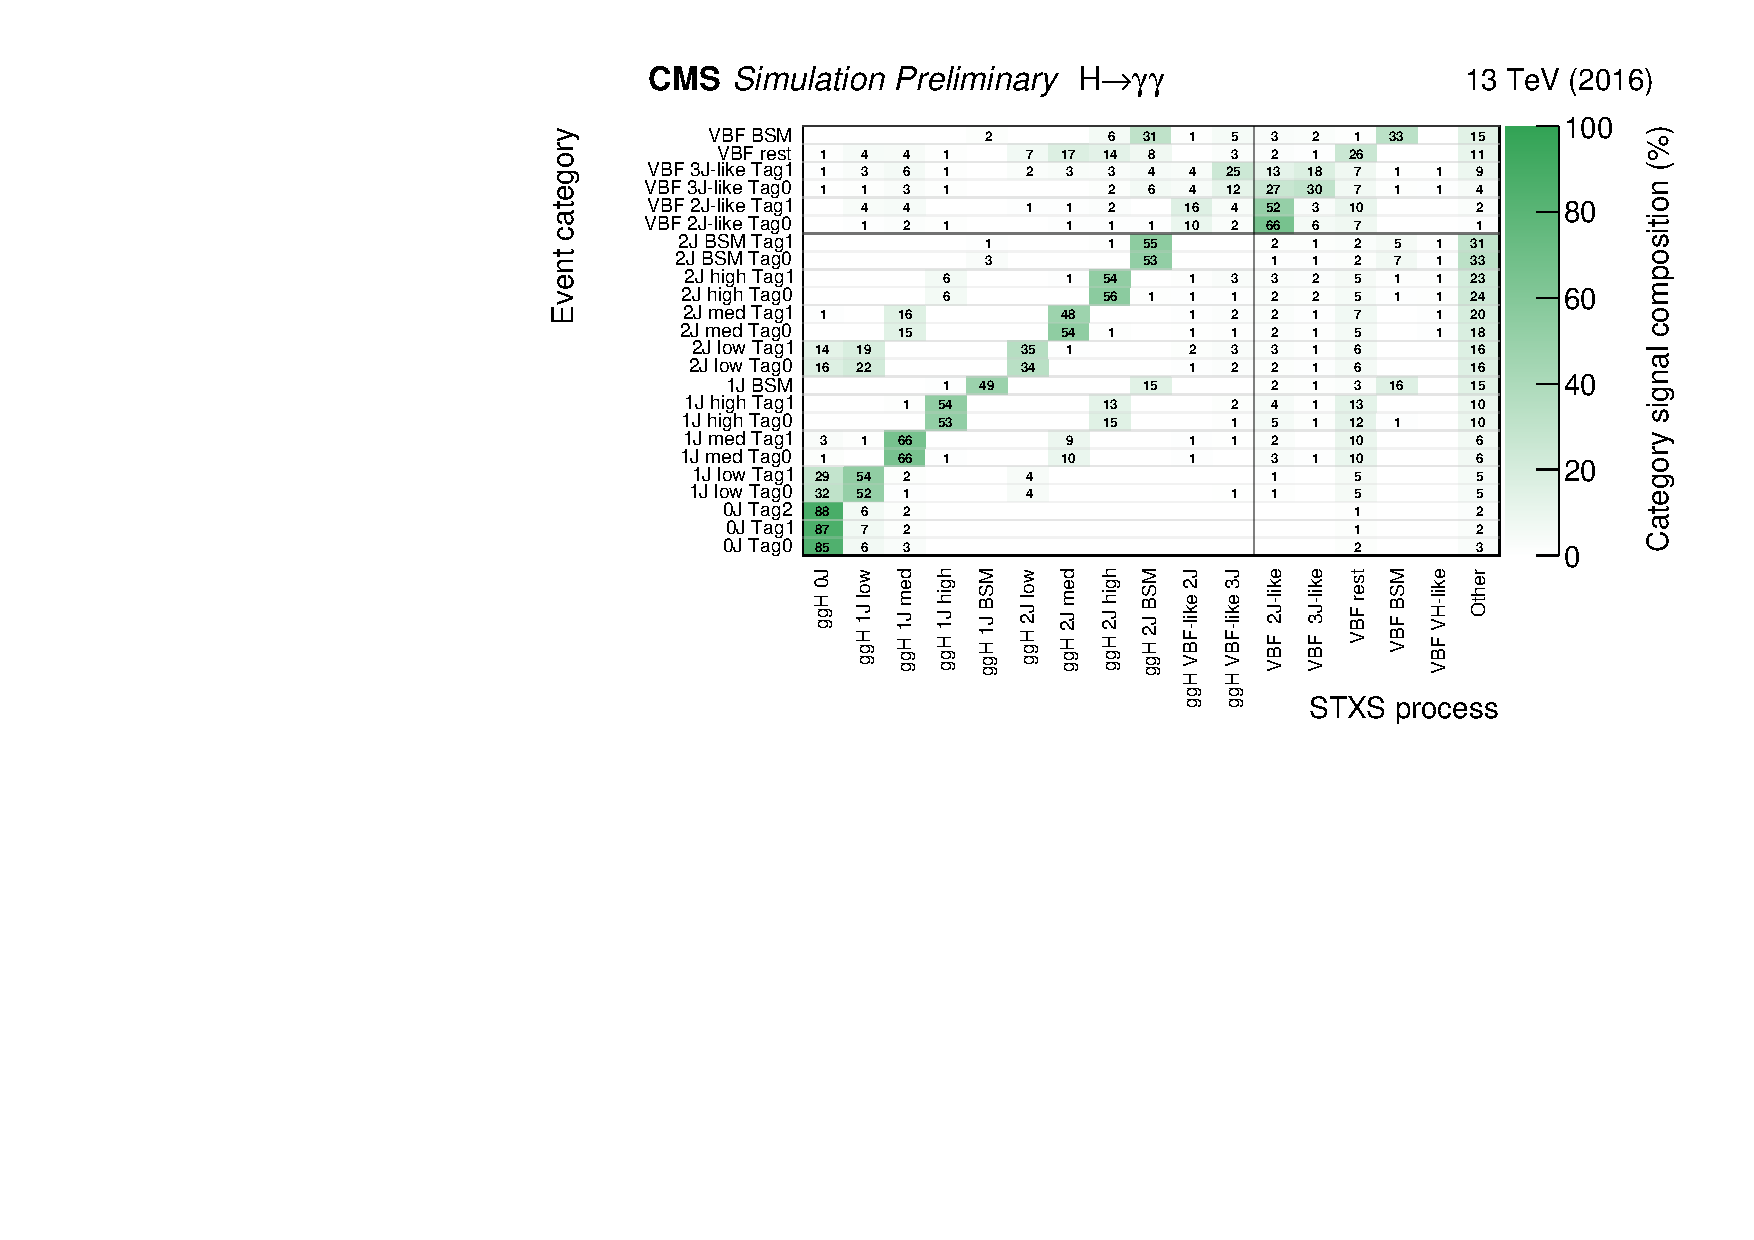
\includegraphics[width=\textwidth]{Figures/Results/Cats2016.pdf}
\caption{
  The composition of each analysis category in terms of stage 1 bins is shown. 
  The colour scale corresponds to the fraction of each category (rows) 
  accounted for by each stage 1 process (columns). 
  Each row therefore sums to 100\%. 
  Entries with values less than 0.5\% are not shown. 
  Simulation corresponding to 2016 conditions is shown.
}
\label{fig:results_Cats2016}
\end{figure}

\begin{figure}[hptb]
\centering
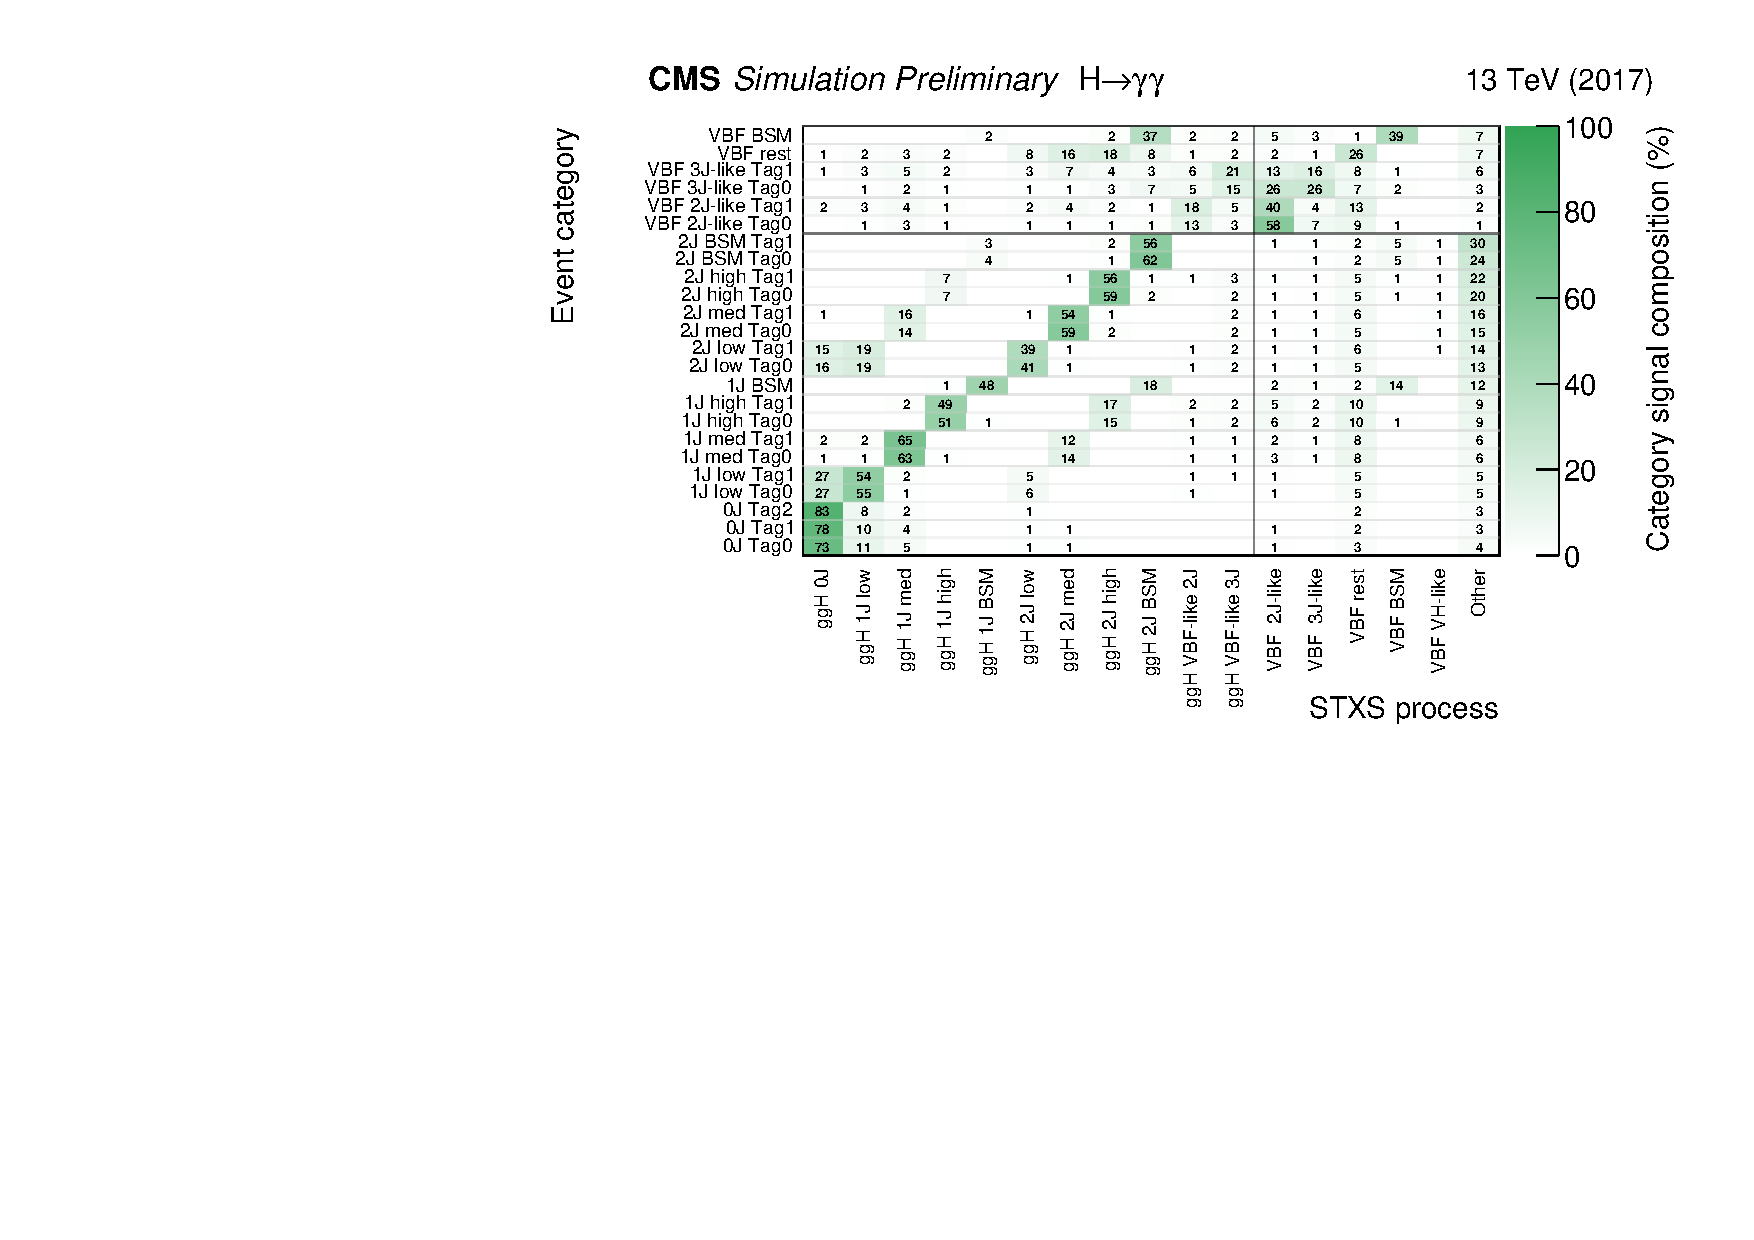
\includegraphics[width=\textwidth]{Figures/Results/Cats2017.pdf}
\caption{
  The composition of each analysis category in terms of stage 1 bins is shown. 
  The colour scale corresponds to the fraction of each category (rows) 
  accounted for by each stage 1 process (columns). 
  Each row therefore sums to 100\%. 
  Entries with values less than 0.5\% are not shown. 
  Simulation corresponding to 2017 conditions is shown.
}
\label{fig:results_Cats2017}
\end{figure}

%TODO insert the big yields tables here

\begin{figure}[hptb]
\centering
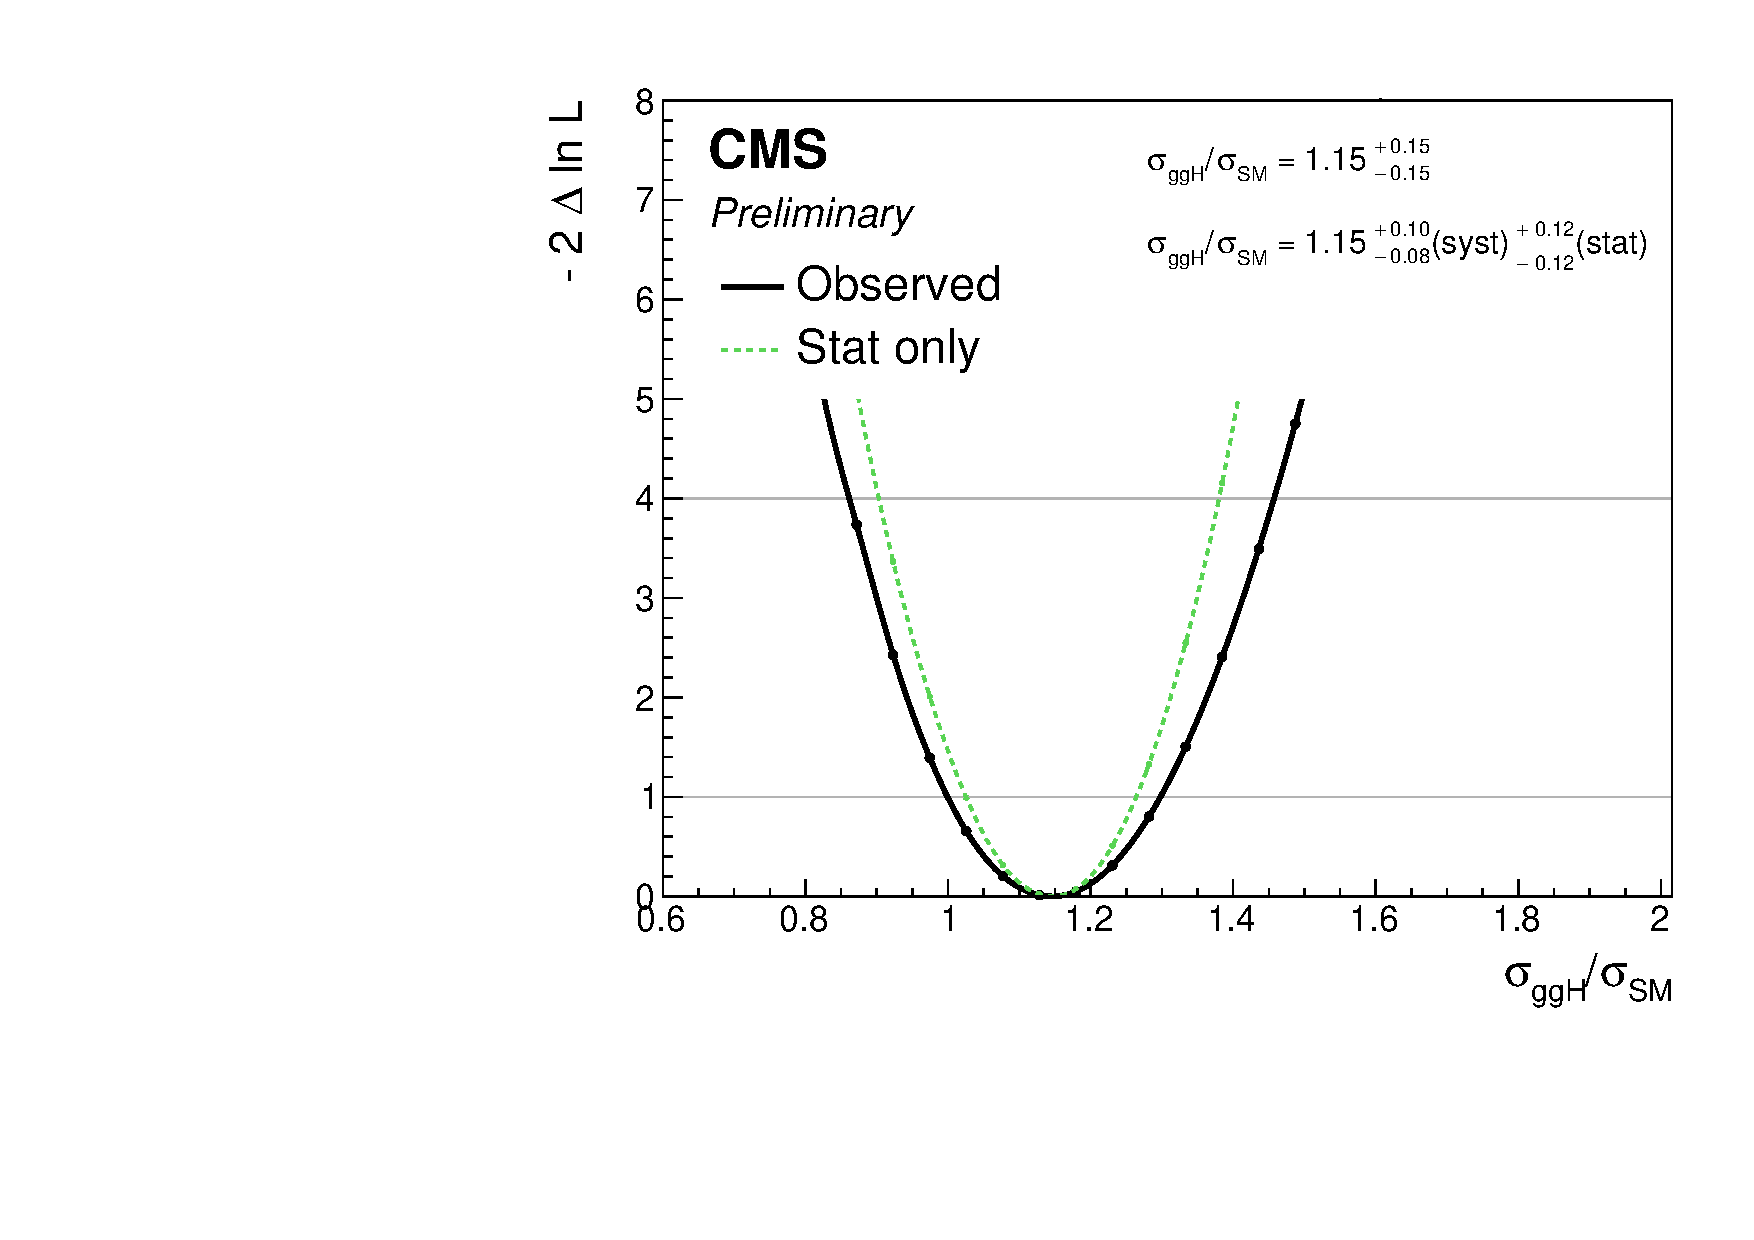
\includegraphics[width=\textwidth]{Figures/Results/ObsStage0_r_ggH.pdf}
\caption{
  The results of a two-parameter fit in the STXS framework,
  showing the scan of the profiled likelihood ratio in the ggH cross section.
  All ggH are grouped together in the fit to form one parameter, 
  with VBF bins comprising the second parameter.
  The ggH parameter includes bbH components, 
  while the qqH parameter includes the hadronic VH contribution. 
  The ttH, tH and VH leptonic processes are constrained to the SM prediction. 
  Cross section ratios are shown with approximate 68\% CL intervals (black points), 
  and compared to the SM expectations and their uncertainties (blue bands).
}
\label{fig:results_Stage0_ggH}
\end{figure}

\begin{figure}[hptb]
\centering
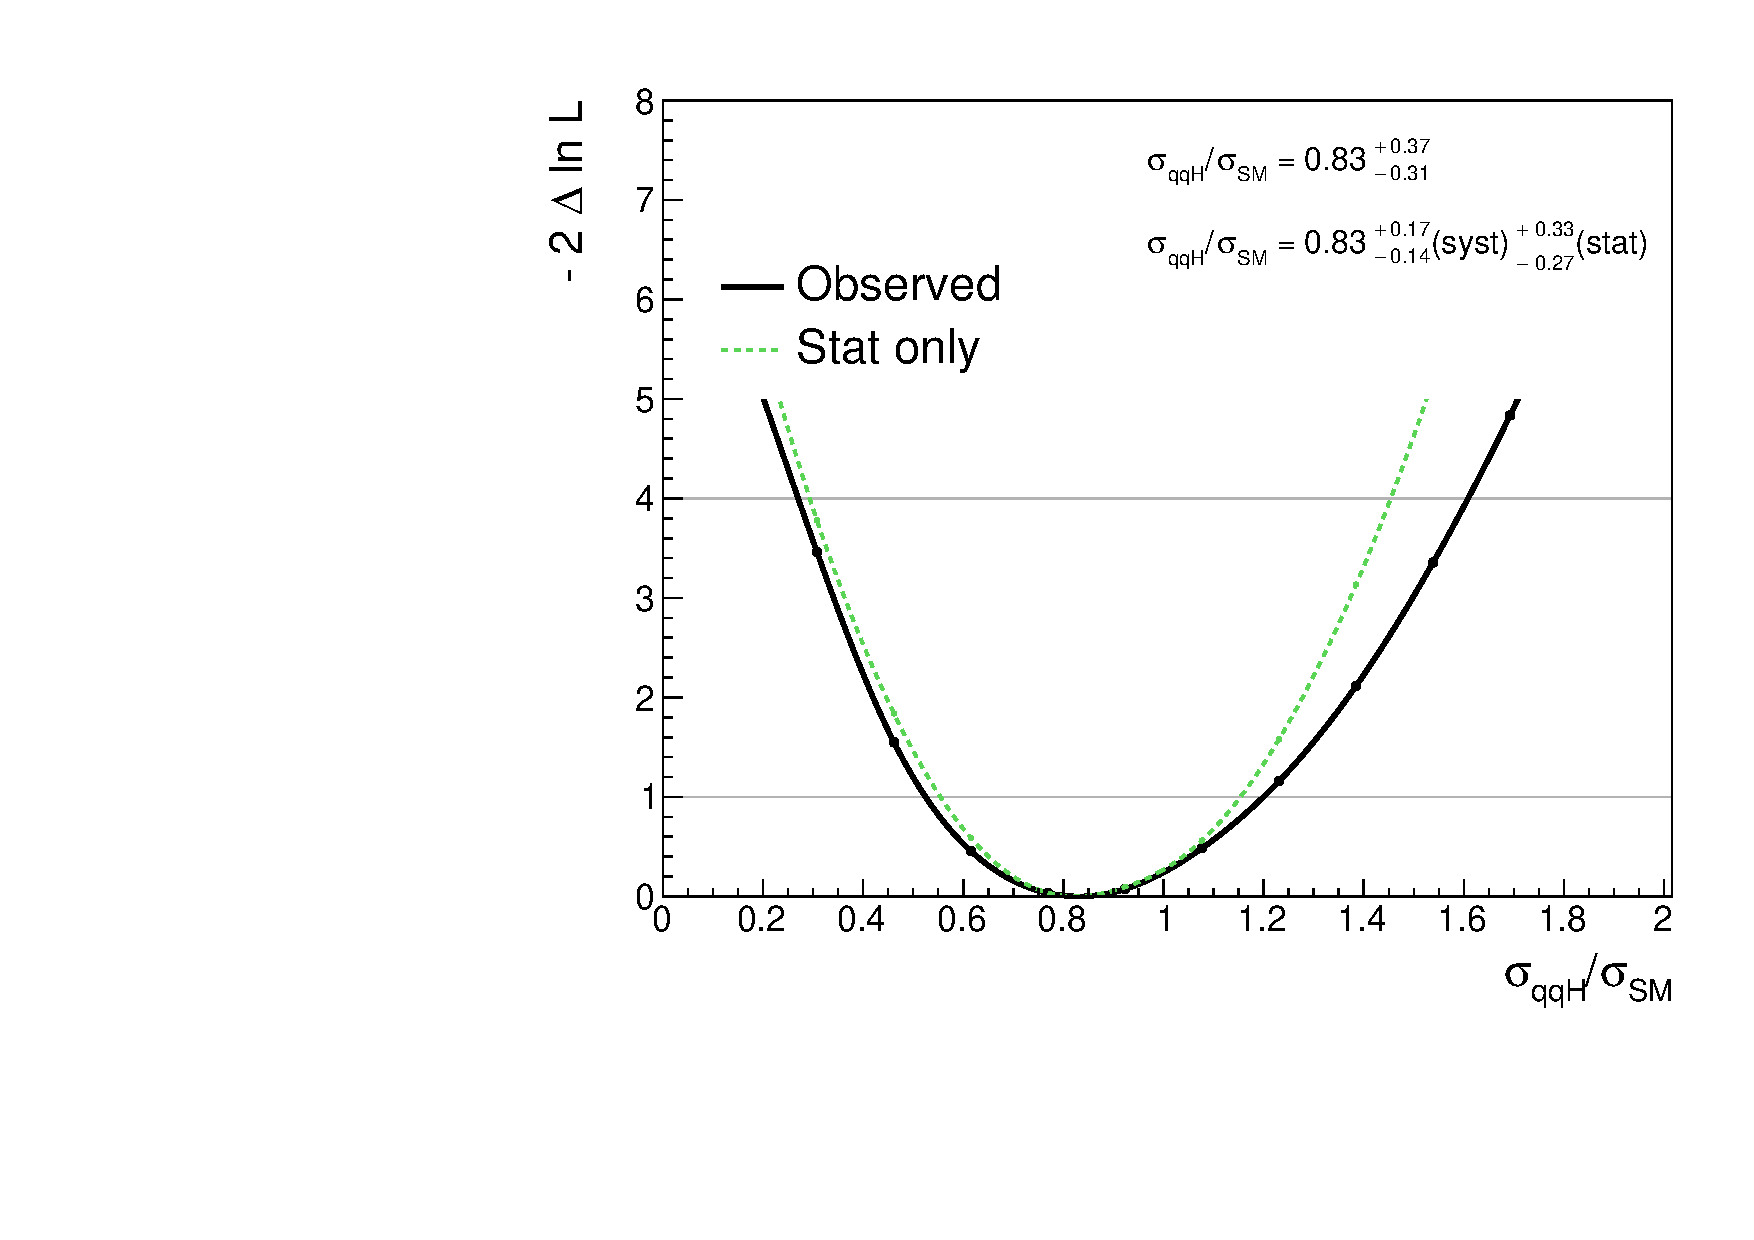
\includegraphics[width=\textwidth]{Figures/Results/ObsStage0_r_qqH.pdf}
\caption{
  The results of a two-parameter fit in the STXS framework,
  showing the scan of the profiled likelihood ratio in the qqH cross section.
  All ggH are grouped together in the fit to form one parameter, 
  with VBF bins comprising the second parameter.
  The ggH parameter includes bbH components, 
  while the qqH parameter includes the hadronic VH contribution. 
  The ttH, tH and VH leptonic processes are constrained to the SM prediction. 
  Cross section ratios are shown with approximate 68\% CL intervals (black points), 
  and compared to the SM expectations and their uncertainties (blue bands).
}
\label{fig:results_Stage0_qqH}
\end{figure}

\begin{figure}[hptb]
\centering
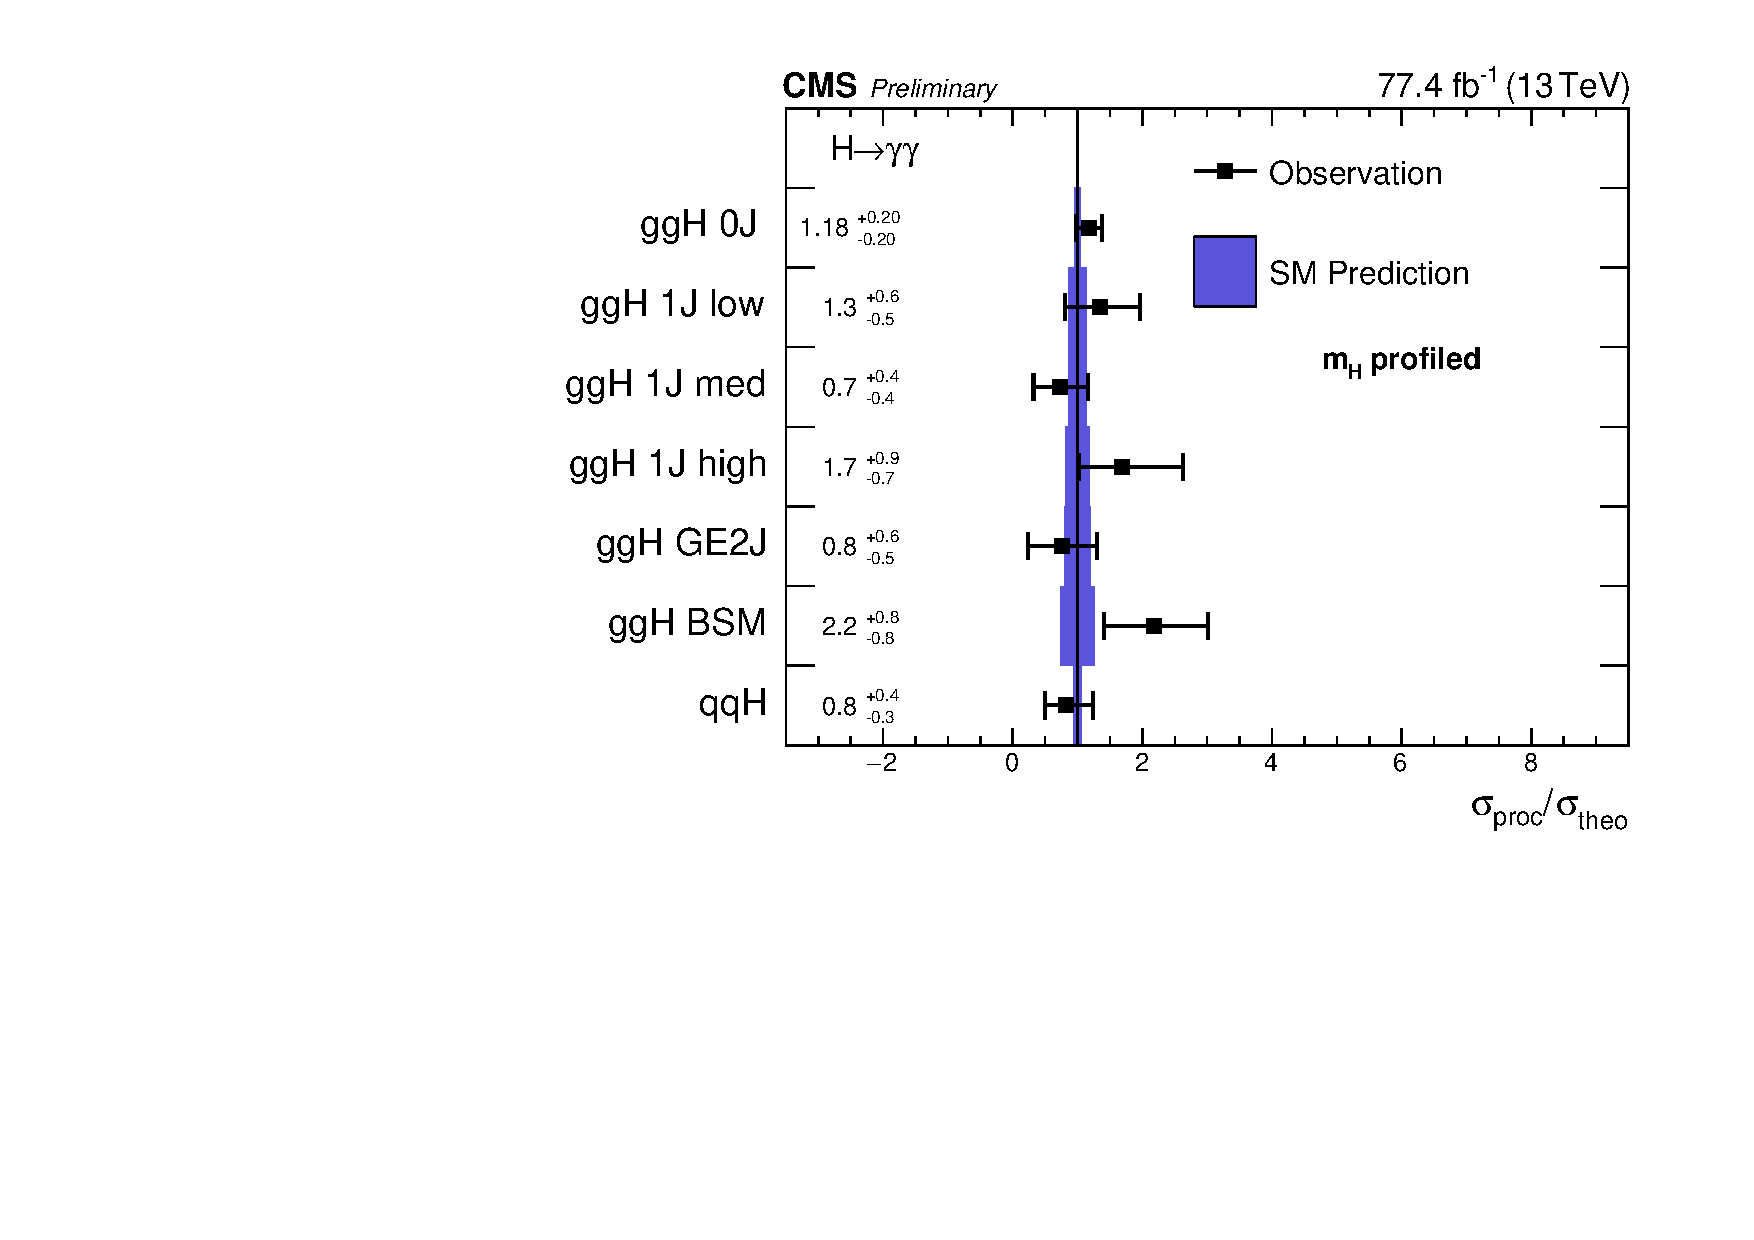
\includegraphics[width=\textwidth]{Figures/Results/Stage1.pdf}
\caption{
  The results of a seven-parameter fit in the STXS framework. 
  The ggH 1J and 2J BSM bins are grouped together in the fit; 
  the remaining five ggH bins with two or more jets are also grouped. 
  All five VBF bins are grouped together. 
  The ggH parameters include bbH components, 
  while the qqH parameter includes the hadronic VH contribution. 
  The ttH, tH and VH leptonic processes are constrained to the SM prediction. 
  Cross section ratios are shown with approximate 68\% CL intervals (black points), 
  and compared to the SM expectations and their uncertainties (blue bands).
}
\label{fig:results_Stage1}
\end{figure}

\begin{figure}[hptb]
\centering
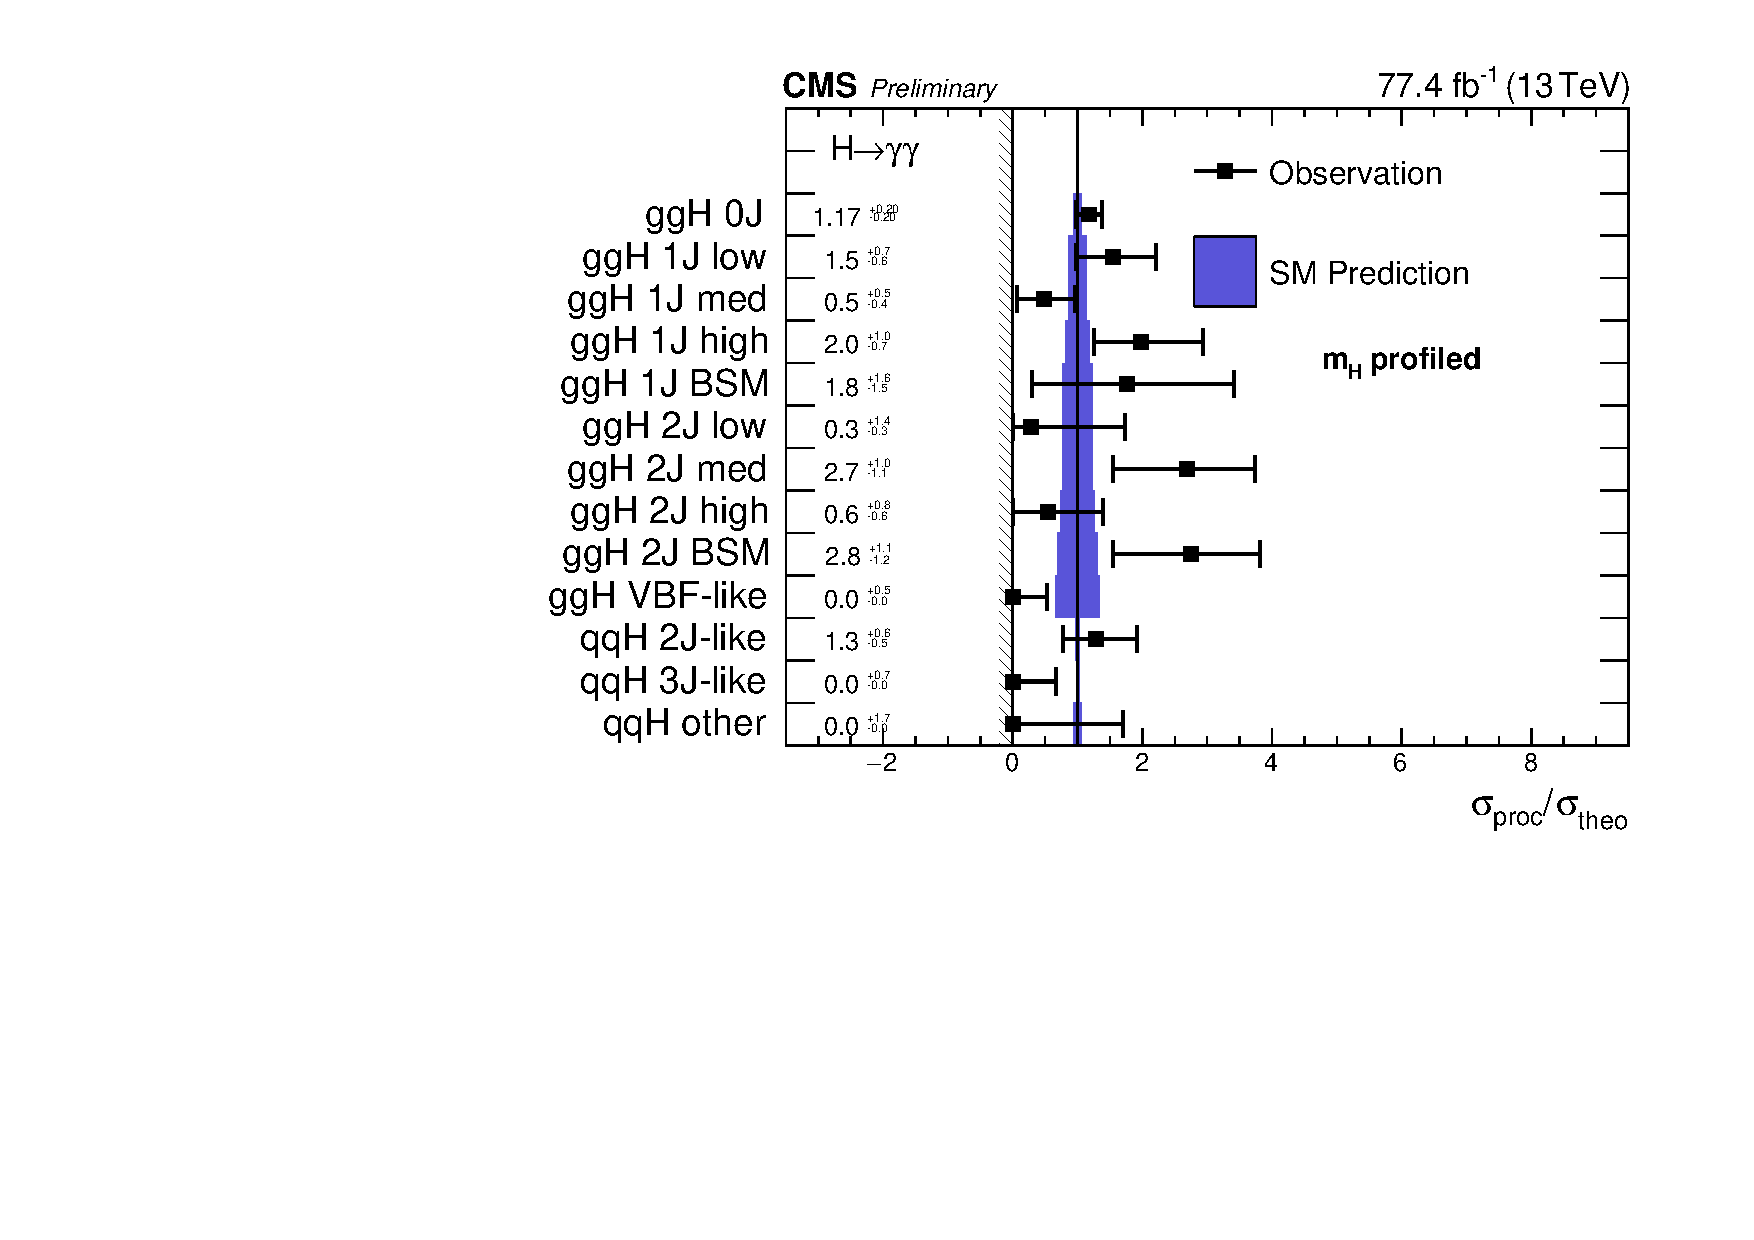
\includegraphics[width=\textwidth]{Figures/Results/Stage1Min.pdf}
\caption{
  The results of a thirteen-parameter fit in the STXS framework. 
  The two VBF-like ggH bins are grouped to form one parameter, 
  as are the VBF BSM-like, VH-like and Rest bins.
  No further merging is performed. 
  The ggH parameters include bbH components, 
  while the qqH parameters include the hadronic VH contribution. 
  The ttH, tH and VH leptonic processes are constrained to the SM prediction. 
  Cross section ratios are shown with approximate 68\% CL intervals (black points) 
  and compared to the SM expectations and their uncertainties (blue bands). 
  The cross section ratios are constrained to be non-negative, 
  as indicated by the vertical line and hashed pattern. 
  The parameters whose best-fit values are at zero are known to have 68\% CL intervals 
  which slightly under-cover; this is checked using pseudo-experiments. 
  The compatibility of this fit with the SM prediction, 
  expressed as a p-value with respect to the SM, is approximately 18\%.
}
\label{fig:results_Stage1Min}
\end{figure}

\begin{figure}[hptb]
\centering
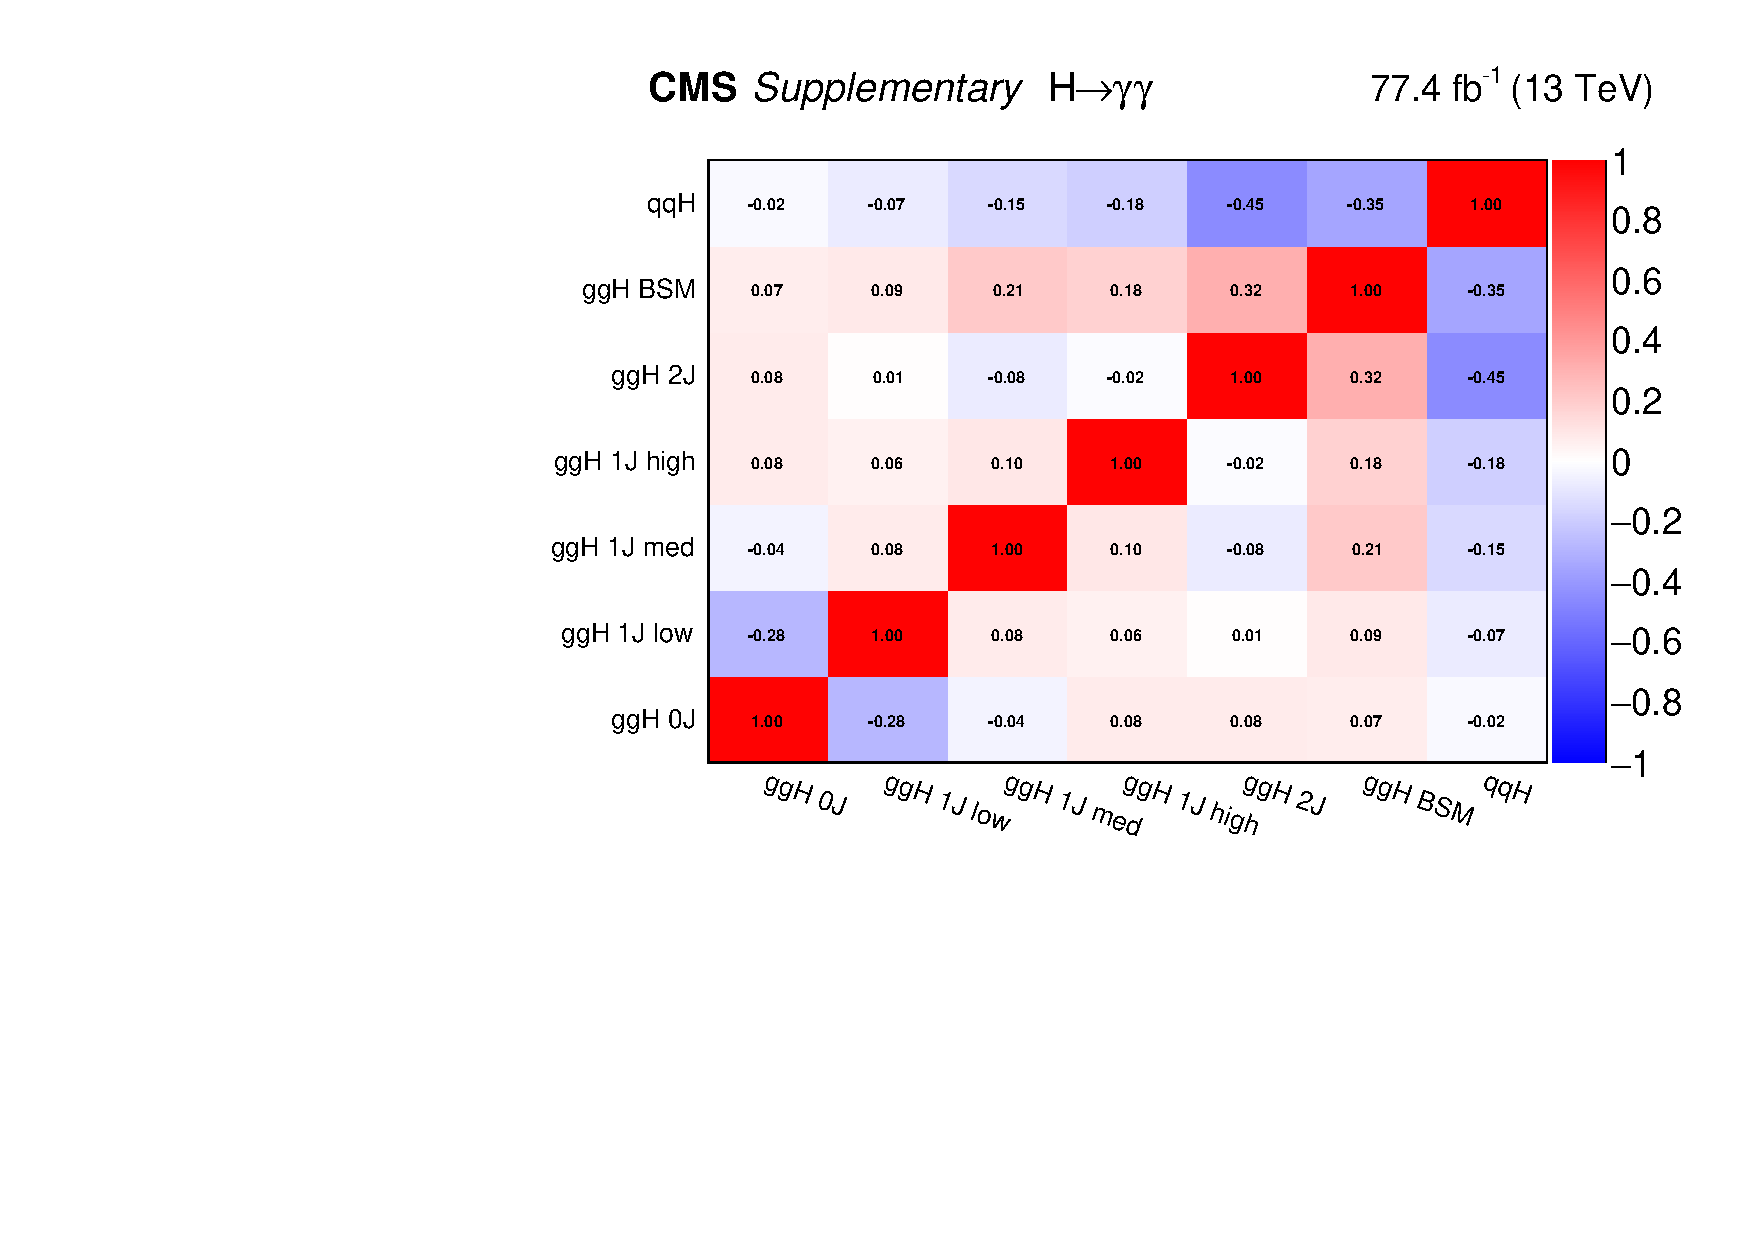
\includegraphics[width=\textwidth]{Figures/Results/CorrStage1.pdf}
\caption{
  Observed correlations in a seven-parameter fit in the STXS framework. 
  The ggH 1J and 2J BSM bins are grouped together in the fit; 
  the remaining five ggH bins with two or more jets are also grouped. 
  All five VBF bins are grouped together. 
  The ggH parameters include bbH components, 
  while the qqH parameter includes the hadronic VH contribution. 
  The ttH, tH and VH leptonic processes are constrained to the SM prediction. 
  The size of the correlation is indicated by the colour scale.
}
\label{fig:results_CorrStage1}
\end{figure}

\begin{figure}[hptb]
\centering
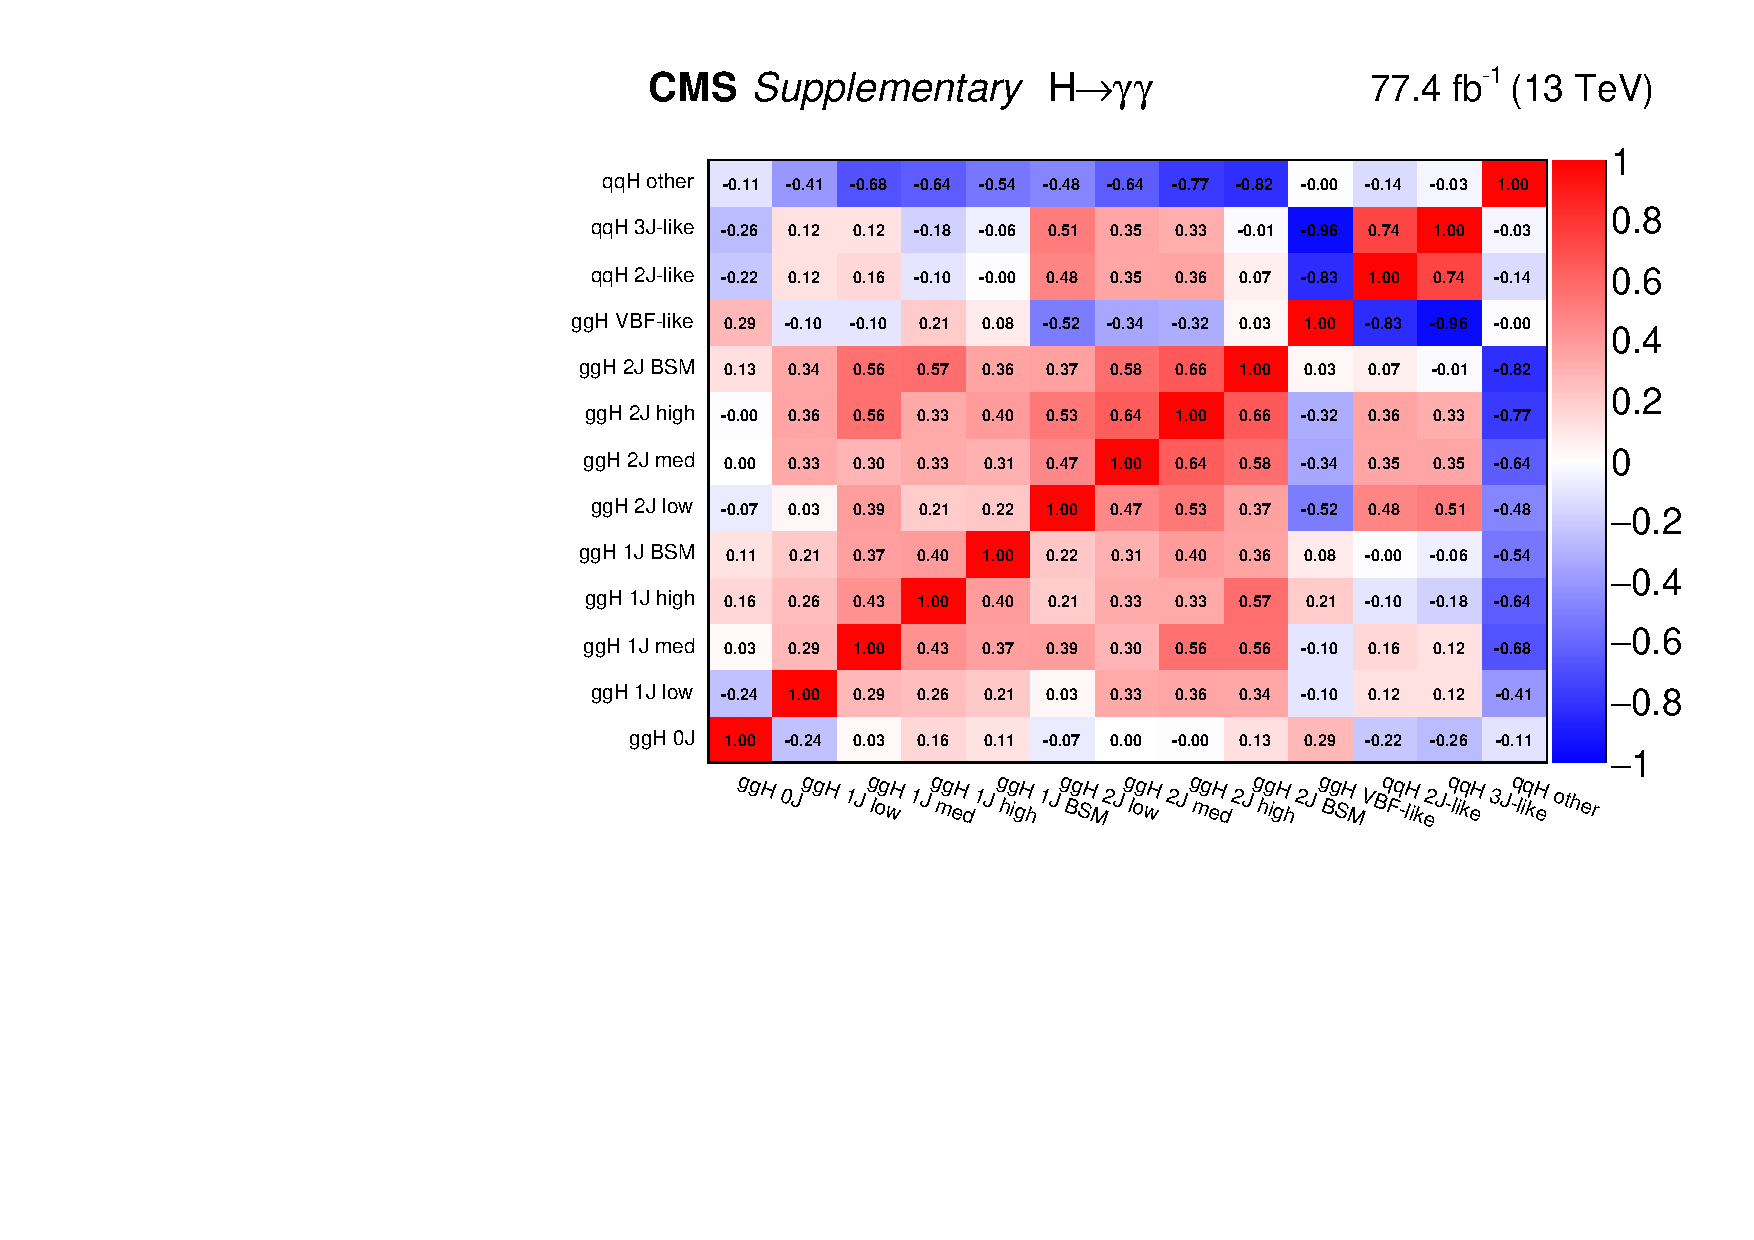
\includegraphics[width=\textwidth]{Figures/Results/CorrStage1Min.pdf}
\caption{
  Observed correlations in a thirteen-parameter fit in the STXS framework. 
  The two VBF-like ggH bins are grouped to form one parameter, 
  as are the VBF BSM-like, VH-like and Rest bins. 
  No further merging is performed. 
  The ggH parameters include bbH components,
  while the qqH parameters include the hadronic VH contribution. 
  The ttH, tH and VH leptonic processes are constrained to the SM prediction. 
  The size of the correlation is indicated by the colour scale.
}
\label{fig:results_CorrStage1Min}
\end{figure}
